\section{Module de croissance du zooplancton}

\subsection{Description du module}
\par{
Dans les travaux pratiques précédents on a analysé la croissance du phytoplancton en fonction des
nutriments disponibles. Dans les modèles actuels nous sommes moins intéressés par l'approvisionnement
alimentaire du phytoplancton. Nous avons plutôt procédé par enquêter l'interaction du phytoplancton avec
un prédateur naturel de cette espèce, le zooplancton. En conséquence le modèle mathèmatique a été simplifié
de manière à ce qu'on considère maintenant une offre des nutriments infiniment grand pour le
phytoplancton\footnote{En d'autres termes, la croissance du phytoplancton n'est plus limitée par les
nutriments}.
\par{
Pour mieux interpréter les simulations du modèle mathématique nous avons émis l'hypothèse que la mortalité
du phytoplancton est uniquement due au broutage du zooplancton. La mortalité du phytoplancton par d'autres
prédateurs, toxines environnementales, lyse cellulaire etc. n'est pas représentée par le modèle.
Nous supposons donc que l'influence de ces causes de mortalité peut être négligée par rapport à l'influence
de la mortalité de phytoplancton due au broutage du zooplancton.
}
\par{
En résumé, nous obtenons le modèle conceptuel effectué dans la figure~\ref{fig:partie1DiagConcept}
et les équations suivantes:
}

\begin{equation}
  {{d[DA]}\over{dt}} =
  \mu_{DA} [DA] - graz_{MSZ} [MSZ]
  \label{eq:partie1DiffEq1}
\end{equation}
\begin{equation}
  {{d[MSZ]}\over{dt}} =
  \left (
    (1- eges_{MSZ}) graz_{MSZ} Y_{MSZ} - mm_{MSZ}
  \right ) [MSZ]
  \label{eq:partie1DiffEq2}
\end{equation}

\par{
Dans la première partie des travaux pratiques, l'intérêt principal est de comparer l'impacte de la
fonctions de broutage. Pour les analyses, les fonctions de broutage suivantes ont été considérées:
}

\begin{equation}
  graz_{MSZ} = g_{MSZ} \max(T) {{[DA]}\over{kg_{MSZ}+[DA]}}
  \label{eq:partie1GrazMic}
\end{equation}
\begin{equation}
  graz_{MSZ} = g_{MSZ} \max(T) {{[DA]-[DA_0]}\over{kg_{MSZ}+([DA]-[DA_0])}}
  \label{eq:partie1GrazMicSeul}
\end{equation}
\begin{equation}
  graz_{MSZ} = g_{MSZ} \max(T) {{[DA]^2}\over{kg_{MSZ}^2+[DA]^2}}
  \label{eq:partie1GrazHol}
\end{equation}

\begin{figure}[h!]
  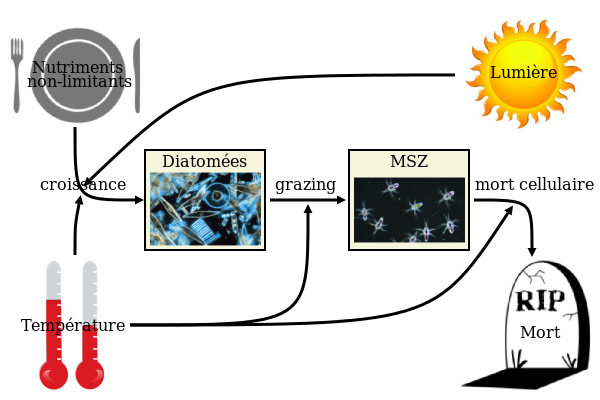
\includegraphics[width=\textwidth]{partie1/diagrammeConceptuel.png}
  \caption{Le modèle conceptuel du système étudié dans le quatrième cours. La croissance du phytoplancton
n'est plus limitée par les nutriments disponibles. Cependant, la croissance est toujours limitée par la
disponibilité de la lumière et de la température. Dans les formules, l'influence de ces deux impacts
environnementals est cachée dans le terme $\mu_{DA}$. Une partie du phytoplancton existant est consommer
par le mésozooplancton (=MSZ). Cette partie est représentée par les fonctions de broutage
différentes fois la concentration du mésozooplancton ($graz_{MSZ}[MSZ]$). Dans le système modèlise
le mésozooplancton n'a pas des prédateurs naturels. La mort cellulaire naturelle du zooplancton ne peut plus
être négligée (dans les formules c'est le terme $mm_{MSZ}$ qui décrit cette l'influence).
}
  \label{fig:partie1DiagConcept}
\end{figure}

\par{

}

\subsection{Analyse mathèmatique}
\subsubsection{États stationnaires}
\par{
La grille~\ref{tab:partie1etatsStat} donne un aperçu des états stationnaires du système
pour les fonctions de broutage differents. Les constantes supplémentaires utilisées
dans la grille sont définies comme suit:
}
\[
m = mm_{MSZ_{MAX_0}} e ^{- \left ( {{t-t_{opt}}\over{d_{opt}}} \right )}
\]
\[
k = kg_{MSZ}
\]
\[
c = \left ( 1 - eges_{MSZ} \right ) y_{MSZ}
g_{MSZ_{MAX_0}} e ^{- \left ( {{t-t_{opt}}\over{d_{opt}}} \right )}
\]
\[
f = g_{MSZ_{MAX_0}} e ^{- \left ( {{t-t_{opt}}\over{d_{opt}}} \right )}
\]

\begin{table}[h!]
\begin{center}
\begin{tabular}{ | c | c c | }
\hline
fct. de broutage & $[DA]$ & $[MSZ]$ \\
\hline
MIC, MIC\_Seul, HOL & 0 & 0 \\
MIC & $k * {{m}\over{c-m}}$ & ${{\mu_{DA} k \left ( 1 + {{m}\over{c-m}} \right )}\over{f}}$ \\
MIC\_Seuil & ${{m/c*k-m/c[DA_0]+[DA_0]}\over{1-m/c}}$ & ${\mu_{DA} * [DA] * (k + [DA] - [DA_0])}\over{f *([DA] - [DA_0])}$ \\
HOL & $k*\sqrt{{{m}\over{c-m}}}$ & ${{\mu_{DA}k \left ( 1 + {m}\over{c-m} \right )}\over{f \sqrt{{m}\over{c-m}}}}$ \\
\hline
\end{tabular}
\end{center}
  \caption{Les états stationnaires du système pour les fonctions de broutage differents.}
  \label{tab:partie1etatsStat}
\end{table}


\subsubsection{Stabilité des états stationnaires}

\subsection{Simulation de référence}

\subsection{Simulation de test 1}

